% Fabian Ehrentraud, 2011-02-03
% Licensed under the Open Software License (OSL 3.0)

%TODO
%fix capitalizations, spelling
%reference to github + javadoc

\def\writedate {February 04, 2011}

\documentclass[12pt,a4paper,titlepage,oneside]{report}


\usepackage{RationalPiano}
\sloppy

\begin{document}
% create titlepage
\maketitle

% tables and lists
\tableofcontents
\newpage
\listoffigures
\newpage
\listoftables
\newpage

% chapters

\chapter{Overview}
\label{chap:overview}

\begin{figure}[htbp]
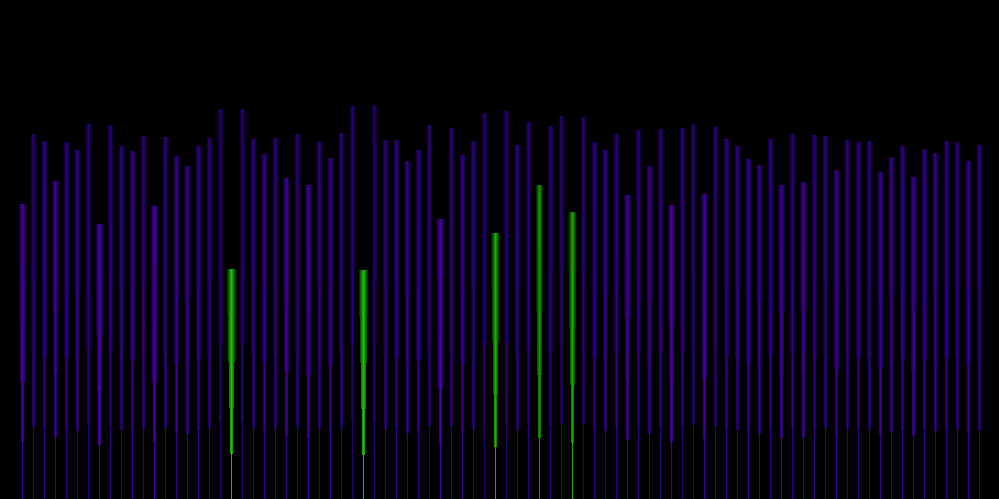
\includegraphics[width=\textwidth]{images/interface_active2.png}
\centering
\caption{The interface of \emph{Rational Piano} in action}
\label{fig:interface_active}
\end{figure}

\begin{figure}[htbp]
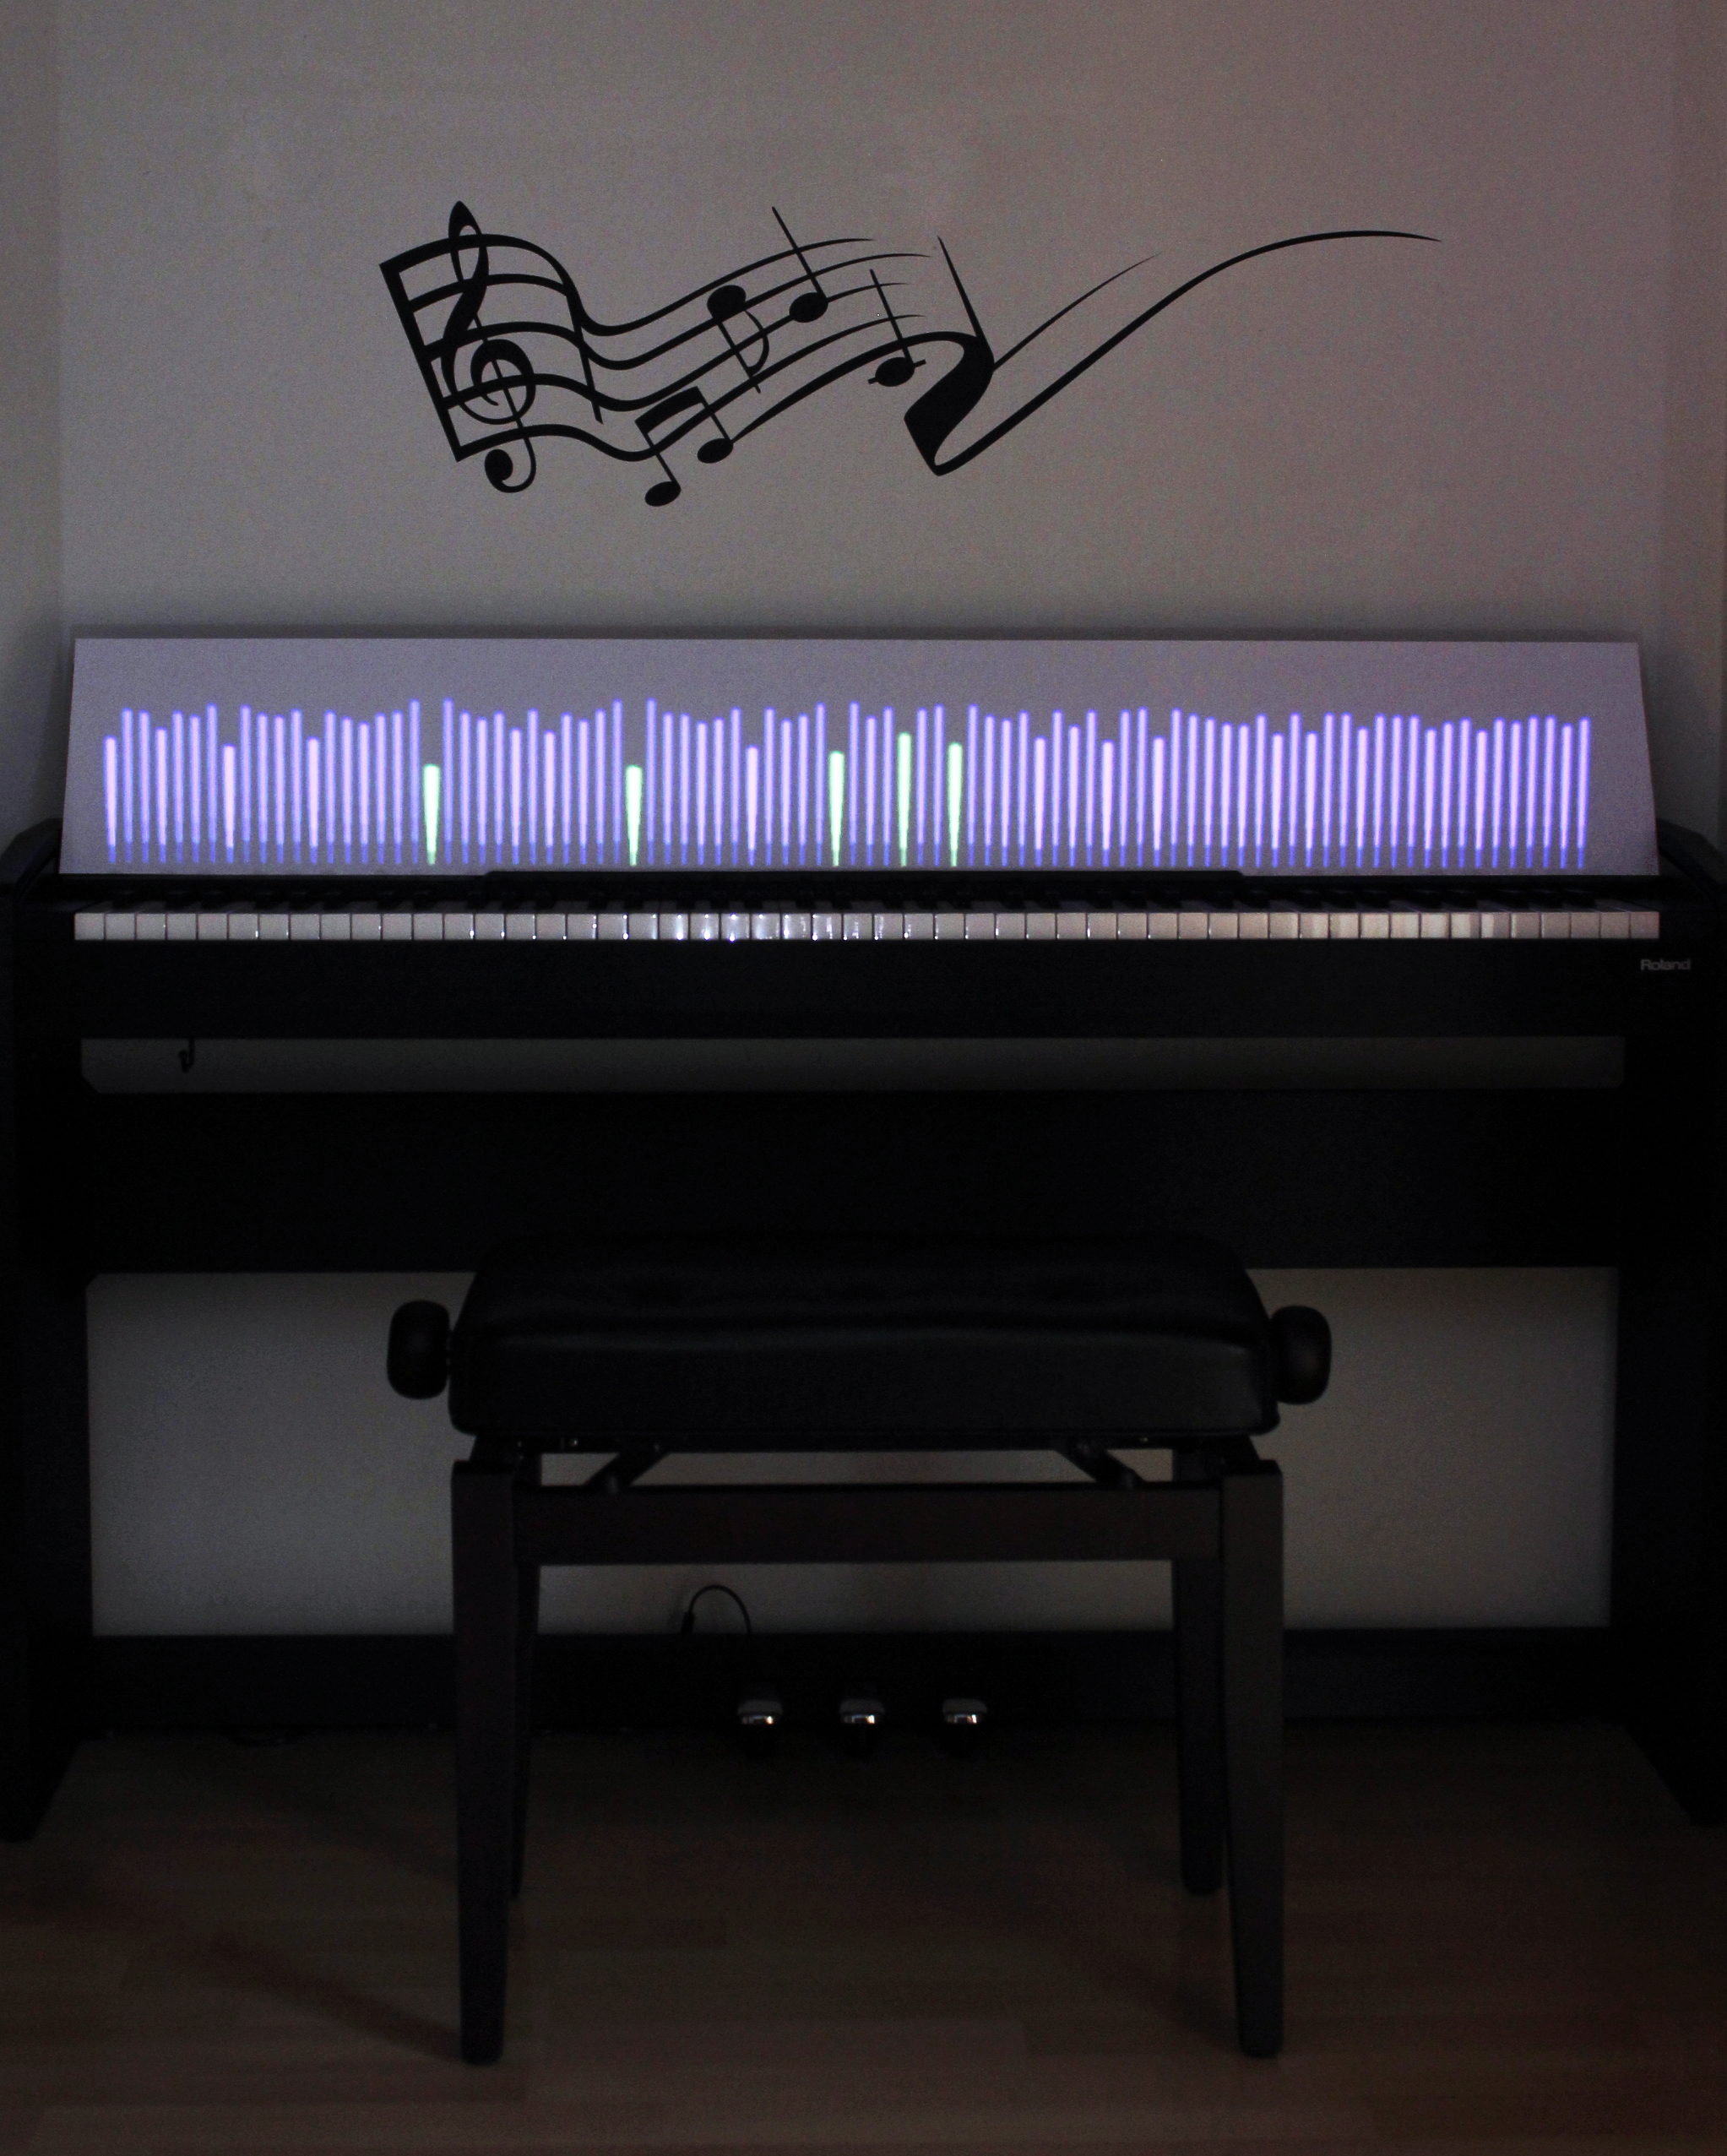
\includegraphics[width=\textwidth]{images/interface_foto.jpg}
\centering
\caption{The interface of a \emph{Rational Piano} installation in action (but without the player)}
\label{fig:interface_foto}
\end{figure}

\emph{Rational Piano} formerly was a piano interface for TUIO~\cite{bib:tuio} enabled multitouch tables. In the current further developed version, the focus was set on different input methods as the used multitouch system had some problems caused by the video input tracking making the system hard to use: high latency, missing pressure detection and also missing tactile feedback. To avoid these problems, now a conventional MIDI\footnote{\emph{MIDI} Wikipedia entry, \url{http://en.wikipedia.org/wiki/Midi}} keyboard is being used as input device.\footnote{TUIO input still is supported}

% Pressing and releasing those lines sends note messages via MIDI or OSC\footnote{with namespace SynOSCopy~\cite{bib:synoscopyNamespace}}~\cite{bib:osc} to external\footnote{external to the \emph{Rational Piano} application, it can still run on the same computer} synthesizer applications.

The system calculates a visualization like shown in Fig.\ref{fig:interface_active} from the MIDI input. For each key on the keyboard\footnote{in the 12TET scale - other scales are planned}, a vertical line is displayed. For all of those lines respectively, the \emph{consonance}\footnote{\label{foot:cons}\emph{Consonance and Dissonance} Wikipedia entry, \url{http://en.wikipedia.org/wiki/Consonance_and_dissonance}} of its corresponding key is visualized by a continuously varying line width and height. Consonance expresses how well each key would fit to the played keys and is calculated in real time with the framerate. The \emph{lower} a line is, the better it should fit to the currently played (and recently released) notes. For an explanation of the thoughts and algorithms behind the consonance calculation, see Chapter~\ref{chap:consonance}. The visualization is optimized for being projected above the fingerboard with a beamer like shown in Fig.\ref{fig:interface_foto}. If you just want to start playing around instantly, you can skip to Chapter~\ref{chap:running}.

\emph{Rational Piano} is open source, and can be found at \url{https://github.com/fabb/Rational-Piano}.

The application was named ``Rational Piano'' because on the one hand, the consonance calculation is based on Rational Numbers and on the other hand, it provides a rational way for playing with melodies and harmonies.


\section{Target Audience}

This application is targeted at \textbf{Musical Novices}.

\emph{Rational Piano} tries to encourage a musical novice to play with the piano instrument without forcing him into doing technical exercises. Rather, it provides an unobtrusive way to show the player harmonious connections while he is playing without the need for understanding the theories behind them. Necessary thinking ballast should be reduced (which tone or chord fits now) and the coupling of the auditive and visual senses should get invigorated. It should be a helping tool to get a feeling for harmonious laws without the need to think about or even to understand the theories behind them. This is also what traditional learning methods aim at but with a higher entry step.


\section{Pictures}

Most of the pictures in this document were drawn with Wolfram Mathematica\textregistered{}~\cite{bib:mathematica}. The source is included in the file \emph{doc/images/images.nb}. The Interaction diagram in Fig.\ref{fig:interaction} was drawn with Dia~\cite{bib:dia}, its source is available in file \emph{doc/images/control\_interaction.dia}.


\section{License}

Source Code, images and other original work including this documentation is licensed under the \textbf{Open Software License version 3.0}~\cite{bib:osl}. The full license text also is available in file \emph{``LICENSE.txt''}.

Libraries in the subfolder ``lib'' are licensed under the original licenses - for more information on these, see Chapter~\ref{sec:libdep}. 


\chapter{Consonance and Dissonance}
\label{chap:consonance}

\section{The Concept}

So what is consonance? There exist many different definitions~\cite{bib:cons_diss}. Consonance expresses how well some sounds fit together. That is dependent of the single sounds' \textbf{base frequencies}, their \textbf{spectra} and also what the listener is \textbf{accustomed} to\footnote{and probably some other things too}. In this application only base frequencies are considered\footnote{If you are interested into spectrum considerations, look up the works of William Sethares~\cite{bib:sethWiki, bib:adaptun}} as it is a good approximation for most harmonic spectra.


\subsection{Ratio of Two Frequencies}

You are probably familiar with the term \emph{Octave}. Imagine (or try out) playing a tone on an instrument like the piano and at the same time play the octave\footnote{In our western music system we most commonly use the \emph{Equal Temperament}~\cite{bib:12tet} which divides one octave into 12 \emph{Semitones}, it is also called \emph{12TET}. So here the octave is 12 Semitones above any tone.} above. Fig.\ref{fig:keyboard_octave} shows playing an A with 440Hz plus its octave above with 880Hz. Playing that \emph{interval} sounds quite good.

\begin{figure}[!ht]
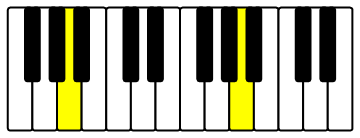
\includegraphics[width=0.5\textwidth]{images/keyboard_octave.png}
\centering
\caption{An \emph{Octave} played on a keyboard, base tone is an A with 440Hz}
\label{fig:keyboard_octave}
\end{figure}

Now, in contrast, play the same first tone and as the second tone use one Semitone \textbf{below} the octave - that interval is called a \emph{Major Seventh}. Fig.\ref{fig:keyboard_major_seventh} shows the keys of that interval where again the lower key is an A with 440Hz and the upper key is a G sharp with (approximately) 825Hz\footnote{Which is a major seventh in Just Intonation~\cite{bib:just}, in 12TET it is actually $440 \cdot 2^{\frac{11}{12}} = 830.609Hz$ which has not got a ratio as it is an irrational number, but we will get to this later}. It does not sound that good anymore\footnote{mileage may vary}, more \textbf{tensionful}, as if the two tones would \textbf{beat} each other.

\begin{figure}[!ht]
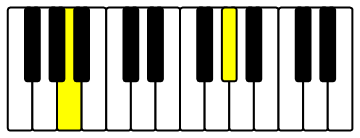
\includegraphics[width=0.5\textwidth]{images/keyboard_major_seventh.png}
\centering
\caption{The interval \emph{Major Seventh} played on a keyboard, base tone is an A with 440Hz}
\label{fig:keyboard_major_seventh}
\end{figure}

So why is that? The (upper) octave of a tone has double its base frequency. So if the lower tone has the (base) frequency $f_{lower}$ and the upper tone has the (base) frequency $f_{higher}$, the simple mathematical relationship is $f_{higher} = 2 \cdot f_{lower}$. The \emph{ratio} of the frequencies is $\frac{f_{higher}}{f_{lower}} = \frac{880Hz}{440Hz} = \frac{2}{1}$. The exact frequencies are of no concern\footnote{as long as we stay in the human hearing range} as they shorten out in the fraction, only the shortened ratio of the frequencies is important. Looking at Fig.\ref{fig:sine_octave} one can see that the two base frequencies ``meet again'' (are in phase) very soon, this fact corrensponds to the low ratio of the frequencies.

\begin{figure}[!ht]
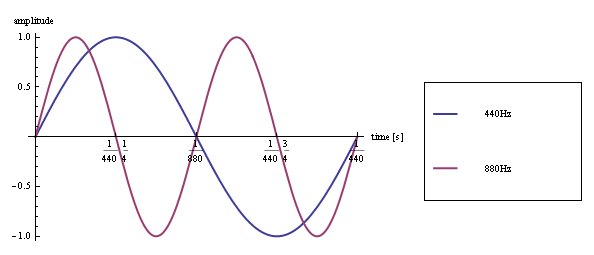
\includegraphics[width=\textwidth]{images/sine_octave.png}
\centering
\caption{Two Sine waves representing the base frequencies $440Hz$ and $880Hz$}
\label{fig:sine_octave}
\end{figure}

Now we look at the second example with the Major Seventh. Here the mathematical relation is $\frac{f_{higher}}{f_{lower}} = \frac{825Hz}{440Hz} = \frac{15}{8}$. In Fig.\ref{fig:sine_major_seventh} one can see that it takes some more cycles for the two base frequencies to ``meet again'' (get in phase), compared to the octave, which corrensponds to the higher ratio of the frequencies.

\begin{figure}[!ht]
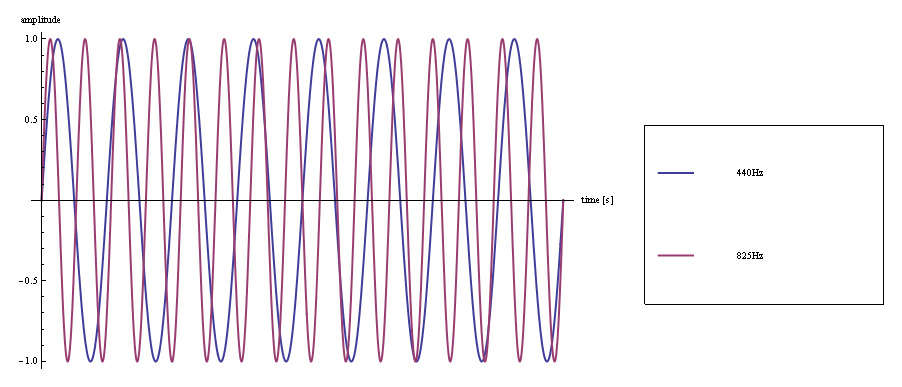
\includegraphics[width=\textwidth]{images/sine_major_seventh.png}
\centering
\caption{Two Sine waves representing the base frequencies $440Hz$ and $\frac{15}{8} \cdot 440Hz = 825Hz$}
\label{fig:sine_major_seventh}
\end{figure}

Comparing those two fractions and more of other intervals shown in Table~\ref{tab:intervals}, one can see that fractions composed of a \textbf{low numerator and denominator} expresses a \textbf{more consonant interval} than a fraction that is composed of a high numerator and/or denominator\footnote{This observation was already made by many, among them Pythagoras~\cite{bib:cons_diss}}. So the lower the result of the \textbf{multiplication of the numerator with the denominator}, the higher the consonance, or in other terms, the lower the dissonance\footnote{Dissonance in this context is used as anti-Consonance, or mathematically $Consonance = \frac{1}{Dissonance}$}.

\noindent
\framebox{
\parbox[][][l]{\textwidth}{
To quantify that mathematically, we can say that $Dissonance(\frac{n}{d}) := n \cdot d$ of the \textbf{shortened} fraction $\frac{n}{d}$, so the \emph{Greatest Common Divisor} of the numerator and denominator is 1: $GCD(n,d) = 1$.
}
}

This function is \emph{commutative} as the multiplication is commutative: $Dissonance(\frac{n}{d}) = n \cdot d = d \cdot n = Dissonance(\frac{d}{n})$.

As all interesting numerator and denominator values are positive and non-zero, the result of the Dissonance fuction will always be at least one. As $Consonance = \frac{1}{Dissonance}$, the result of the Consonance function will always lie between 0 and 1.

\begin{table}[ht]
\renewcommand*\arraystretch{1.5}
\centering
\begin{tabular}{| c | l | c | c |}
\hline
Number of Semitones & Interval Name  &	Just Intonation & Equal Temperament   \\ \hline
0                   & unison         & $\frac{1}{1}$    & $2^{\frac{0}{12}}$  \\ \hline
1                   & semitone       & $\frac{16}{15}$  & $2^{\frac{1}{12}}$  \\ \hline
2                   & whole tone     & $\frac{9}{8}$    & $2^{\frac{2}{12}}$  \\ \hline
3                   & minor third    & $\frac{6}{5}$    & $2^{\frac{3}{12}}$  \\ \hline
4                   & major third    & $\frac{5}{4}$    & $2^{\frac{4}{12}}$  \\ \hline
5                   & perfect fourth & $\frac{4}{3}$    & $2^{\frac{5}{12}}$  \\ \hline
6                   & tritone        & $\frac{7}{5}$    & $2^{\frac{6}{12}}$  \\ \hline
7                   & perfect fifth  & $\frac{3}{2}$    & $2^{\frac{7}{12}}$  \\ \hline
8                   & minor sixth    & $\frac{8}{5}$    & $2^{\frac{8}{12}}$  \\ \hline
9                   & major sixth    & $\frac{5}{3}$    & $2^{\frac{9}{12}}$  \\ \hline
10                  & minor seventh  & $\frac{9}{5}$    & $2^{\frac{10}{12}}$ \\ \hline
11                  & major seventh  & $\frac{15}{8}$   & $2^{\frac{11}{12}}$ \\ \hline
12                  & octave         & $\frac{2}{1}$    & $2^{\frac{12}{12}}$ \\ \hline
\end{tabular}
\caption{Intervals in an octave and their ratios according to Just Intonation and non-rational multiples according to Equal Temperament}
\label{tab:intervals}
\end{table}


\subsection{Inexact Fractions}
%TODO more clear wording
While working with rational numbers now seems easy, we have got a \textbf{problem} when working with ratios of the Equal Temperament. As you can see in Table~\ref{tab:intervals}, its tones' ratios consist of roots of the number two. All of those (exept to octaves) are \emph{Irrational Numbers} that have got \textbf{no fractional representation}. That means if we have given any two frequencies that have no rational ratio, in the mathematic sense, we can not calculate the consonance.

Even with perfect ratios, there is a \textbf{problem}: if there are two tones playing with a ratio that has got a high numerator and denominator, and therefore a high dissonance, it still could be that the interval sounds consonant. That is the case if there is a nearby fraction with a low numerator and denominator. As you can see in Fig.\ref{fig:enharmonic}, the two ratios are just (approximately) 1 \emph{Cent}\footnote{1 Cent equals the ratio $2^{\frac{1}{1200}}$~\cite{bib:cent}.} apart, which is the lower bound of hearing difference of the human's ear, meaning the \textbf{two ratios cannot be distinguished} even though their dissonances differ about many orders of magnitude.

\noindent
\framebox{
\parbox[][][l]{\textwidth}{
The human ear tends to hear more consonant ratios, even if they are some cent apart.
}
}

But the farther apart, the less good it sounds.

\begin{figure}[!ht]
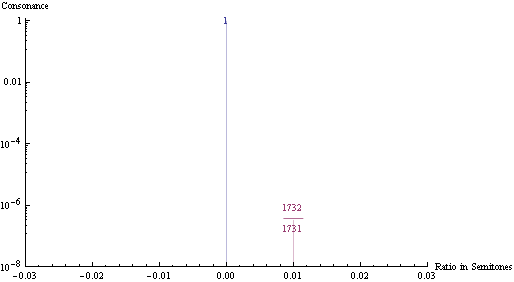
\includegraphics[width=\textwidth]{images/enharmonic.png}
\centering
\caption{Nearby ratios that are indistinguishable}
\label{fig:enharmonic}
\end{figure}

To both fill the ``irrational holes'' and take proximate and more consonant fractions into consideration, each fraction gets ``fuzzified'' by a \emph{Gaussian Bell Curve} like shown in Fig.\ref{fig:bellcurve}~\cite{bib:bell}. In Fig.\ref{fig:just_bell} you can see all ratios from Just Intonation with a bell curve around them. Note that the left half of the figure was added by taking the inverse of every ratio. You can see that consonance calculation of a ratio is a commutative function as it is symmetric.

\begin{figure}[!ht]
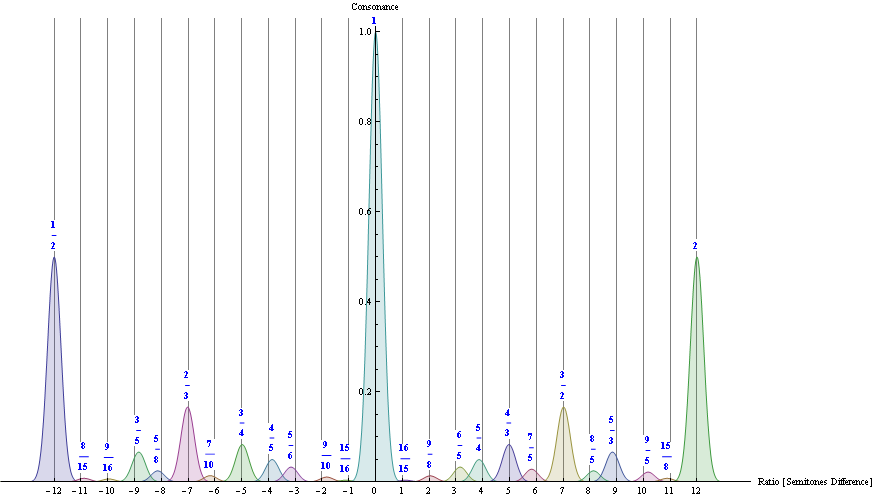
\includegraphics[width=\textwidth]{images/just_bell.png}
\centering
\caption{The ``fuzzified'' Ratios of Just Intonation from Table~\ref{tab:intervals}, note that there was added an octave below by taking the inverse of each fraction}
\label{fig:just_bell}
\end{figure}

To get the heard fraction for any given (maybe irrational) ratio, the maximum consonance of every point on the ratio axis is taken like seen in Fig.\ref{fig:just_bell_max}.

To get the \emph{Semitone Difference} between two tones, the formula $12 \cdot log_2(\frac{f_1}{f_2})$ is used\footnote{Later, when calculating the consonances, the absolute value will be taken as the curve is symmetric and only one side is needed}.

\begin{figure}[!ht]
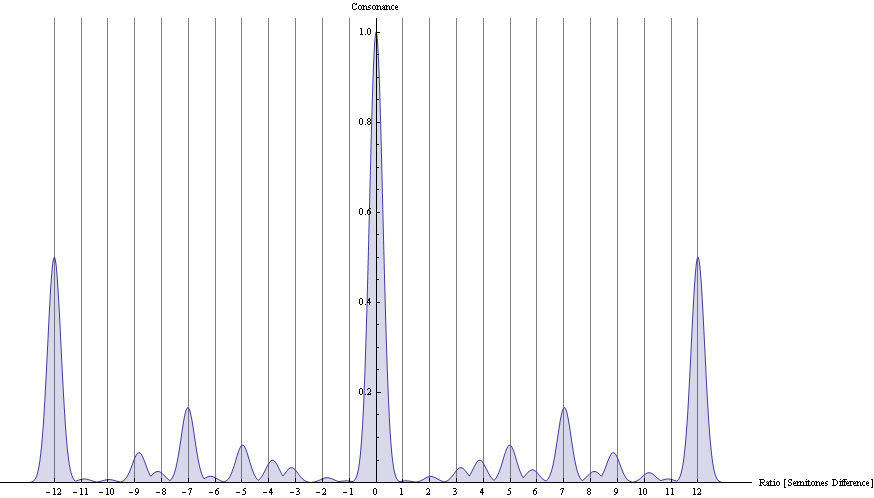
\includegraphics[width=\textwidth]{images/just_bell_max.png}
\centering
\caption{The Maximum Consonance of each Point on the Ratio Axis is heard, so this is the only interesting value}
\label{fig:just_bell_max}
\end{figure}


\subsection{Considered Fractions}

The consonance curve of the last section allows to calculate the consonance of any two sounding tones\footnote{with equal volume, but more about that later} with given base frequencies, considering the fractions of Just Intonation.

But there are more interesting (meaning more consonant) fractions than those in Just Intonation. How to calculate those?

According to the formula 
\[Dissonance(\frac{n}{d}) = n \cdot d : GCD(n,d) = 1\]
there exists at least one fraction for \textbf{any integer value} of the Dissonance function. We are only interested in positive non-zero results (and numerators and denominators) as negative, zero and infinite frequency values do not make much sense\footnote{here}. The first few Dissonance values with their according fractions are listed in Table~\ref{tab:dissonances}.

\begin{table}[ht]
\renewcommand*\arraystretch{1.5}
\centering
\begin{tabular}{| l | l |}
\hline%XXXtable width and first row height
\parbox[][][l]{0.5\textwidth}{\vspace{5pt} Dissonance Value \\ and its prime factorization \vspace{5pt}} & \parbox[][][l]{0.5\textwidth}{\vspace{5pt} Shortened Fractions \\ and their prime factorizations \vspace{5pt}} \\ \hline
$1$                                          & $\frac{1}{1}$                                      \\ \hline
$2$                                          & $\frac{2}{1}$, $\frac{1}{2}$                       \\ \hline
$3$                                          & $\frac{3}{1}$, $\frac{1}{3}$                       \\ \hline
$4 = 2^2$                                    & $\frac{4}{1}$ = $\frac{2^2}{1}$, $\frac{1}{4}$ = $\frac{1}{2^2}$ \\ \hline
$5$                                          & $\frac{5}{1}$, $\frac{1}{5}$                       \\ \hline
$6 = 2 \cdot 3$                              & $\frac{6}{1}$ = $\frac{2 \cdot 3}{1}$, $\frac{3}{2}$, $\frac{2}{3}$, $\frac{1}{6}$ = $\frac{1}{2 \cdot 3}$ \\ \hline
$7$                                          & $\frac{7}{1}$, $\frac{1}{7}$                       \\ \hline
$8 = 2^3$                                    & $\frac{8}{1}$ = $\frac{2^3}{1}$, $\frac{1}{8}$ = $\frac{1}{2^3}$ \\ \hline
$9 = 3^2$                                    & $\frac{9}{1}$ = $\frac{3^2}{1}$, $\frac{1}{9}$ = $\frac{1}{3^2}$ \\ \hline
$10 = 2 \cdot 5$                             & $\frac{10}{1}$ = $\frac{2 \cdot 5}{1}$, $\frac{5}{2}$, $\frac{2}{5}$, $\frac{1}{10}$ = $\frac{1}{2 \cdot 5}$ \\ \hline
$11$                                         & $\frac{11}{1}$, $\frac{1}{11}$                       \\ \hline
$12 = 2^2 \cdot 3$                           & $\frac{12}{1}$ = $\frac{2^2 \cdot 3}{1}$, $\frac{4}{3}$ = $\frac{2^2}{3}$, $\frac{3}{4}$ = $\frac{3}{2^2}$, $\frac{1}{12}$ = $\frac{1}{2^2 \cdot 3}$ \\ \hline
\end{tabular}
\caption{All (positive non-zero) Dissonance Values with their corresponding Fractions and their Prime Factorization}
\label{tab:dissonances}
\end{table}

Examining the shortened fractions and their prime factorizations~\cite{bib:factorization}, one can see that all prime facors of the Dissonance value are distributed on each side of the fraction bar. Each prime factor stays with its powers, e.g. a $3^2$ will be placed either in the numerator or the denominator, but it will not get torn apart into $\frac{3 \cdot x}{3 \cdot y}$ as that would shorten out and lead to a lower Dissonance value\footnote{that has already been covered by the emerging algorithm}. For the prime factors of the Dissonance value, \emph{all possibilities} of putting its prime factors on the left or right side of the fraction bar are exploited.

That way, given a maximum wanted Dissonance value\footnote{called \emph{maxfrac} in the settings of Rational Piano~\ref{sec:ADSR}}, we can calculate all fractions that are more consonant than this. In Fig.\ref{fig:maxfrac_fractions}, all fractions with a Dissonance value lower or equal to \emph{157} are shown. As the numbers collide a lot, Fig.\ref{fig:maxfrac_fractions_log} shows the same fractions in a logarithmical measure.

\begin{figure}[!ht]
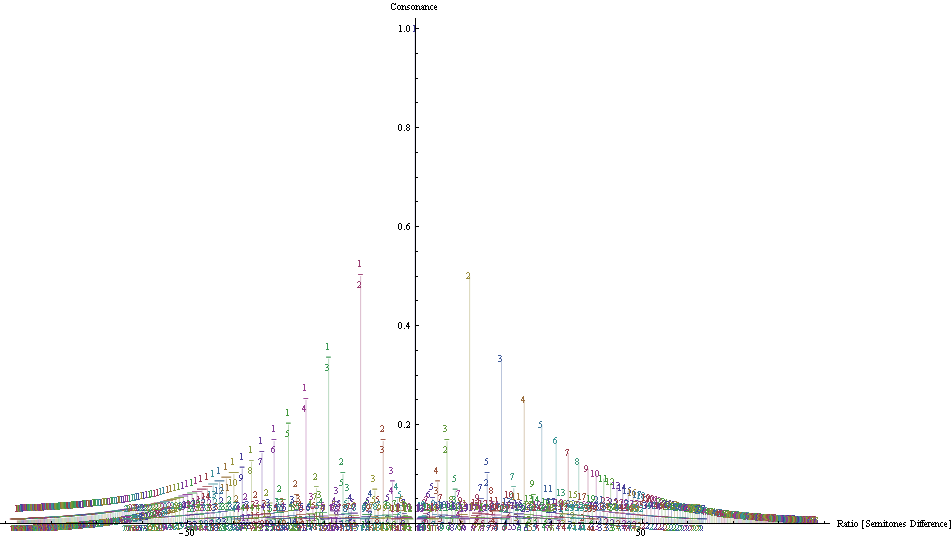
\includegraphics[width=\textwidth]{images/maxfrac_fractions.png}
\centering
\caption{All Fractions with a Dissonance value lower or equal to 157}
\label{fig:maxfrac_fractions}
\end{figure}

\begin{figure}[!ht]
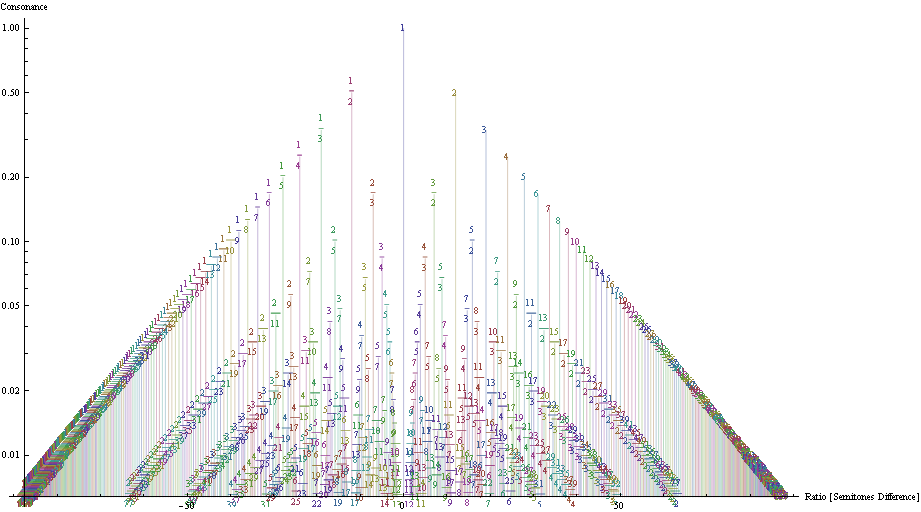
\includegraphics[width=\textwidth]{images/maxfrac_fractions_log.png}
\centering
\caption{All Fractions with a Dissonance value lower or equal to 157 in a Logarithmical Measure}
\label{fig:maxfrac_fractions_log}
\end{figure}

As we have noticed earlier, the Dissonance Function is commutative, thus we can ignore the left side of the plot when we take the absolute value of the semitone difference instead.

In the same way as in the last section, we can now ``fuzzify'' each fraction with a bell curve and then, for each point on the ratio axis, calculate the maximum consonance. Fig.\ref{fig:maxfrac_maxbell} shows the result and Fig.\ref{fig:maxfrac_maxbell_log} the same with a logarithmical measure. Both only show a part of the the right half of the full range.

The \emph{Harmonic Entropy Model}~\cite{bib:harmonic_entropy} is based on similar thoughts and leads to a very similar figure.

\begin{figure}[!ht]
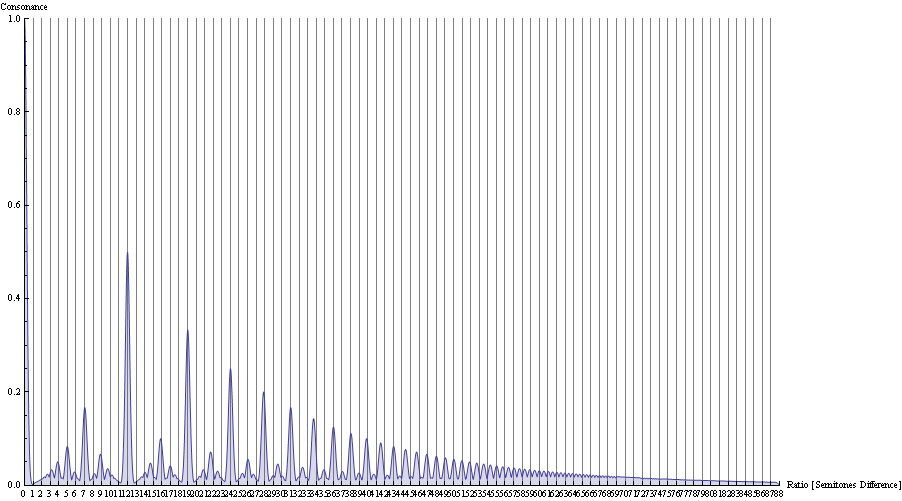
\includegraphics[width=\textwidth]{images/maxfrac_maxbell.png}
\centering
\caption{Consonance for Frequency Ratios of up to 4 Octaves}
\label{fig:maxfrac_maxbell}
\end{figure}

\begin{figure}[!ht]
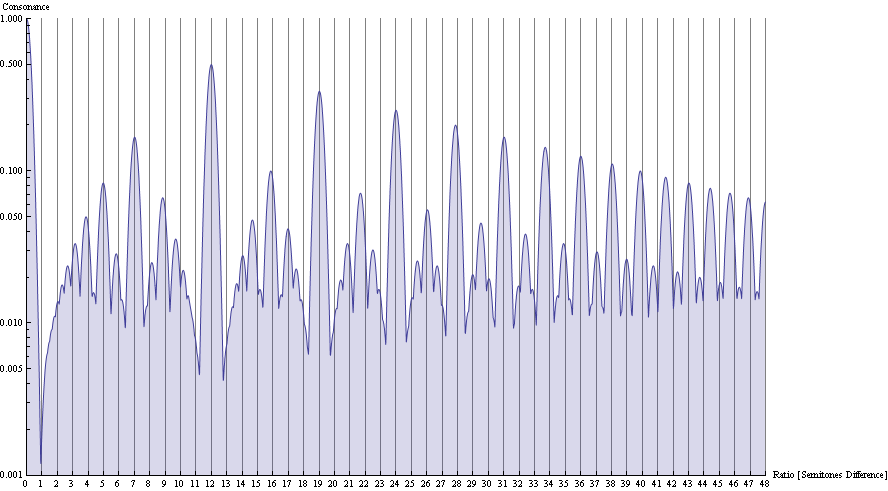
\includegraphics[width=\textwidth]{images/maxfrac_maxbell_log.png}
\centering
\caption{Consonance for Frequency Ratios of up to 4 Octaves in a Logarithmical Measure}
\label{fig:maxfrac_maxbell_log}
\end{figure}

The Dissonance of any two arbitrary frequencies then is:

$
DissonanceF(frequency_1,frequency_2) := \\
DissonanceCurve(12 \cdot log_2(\frac{frequency_1}{frequency_2})) = \\
DissonanceCurve(| 12 \cdot log_2(\frac{frequency_1}{frequency_2}) |)
$ %TODO fix visual appearance

The logarithm translates the frequency ratio to a semitone difference.


\smallskip
\smallskip
\noindent
\framebox{
\parbox[][][l]{\textwidth}{
Calculating the ratio which has its maximum for each step of equal temperament within the first octave leads to an interesting result: it is exactly the corresponding interval in just intonation seen in Table~\ref{tab:intervals} in the same row respectively. The calculation is left out as it would go beyond the scope of this bachelor's thesis.
}
}
\smallskip


\subsection{Taking Account for the Tones' Volumes}

With the calculated curves from the previous section, it is possible to calculate the consonance of any two frequencies \textbf{with the same volumes}. To grasp why this is, imagine two very dissonant tones playing with the same volume. When one of the two gets quieter and the other stays at its volume level, the perceived dissonance vanishes as the quieter tone does not ``disturb'' the louder one anymore.

Assuming the tone's volumes are in the range $[0,1]$\footnote{For real tones, there is no upper limit on the volume, but for the calculation stated here, they would have to get cropped or scaled.}, we can multiply the calculated Dissonance value with the two volumes which makes it smaller and thus makes the Consonance value bigger:

$
DissonanceFV(frequency_1,volume_1,frequency_2,volume_2) := \\
Dissonance(volume_1 \cdot volume_2 \cdot DissonanceF(frequency_1,frequency_2))
$ %TODO fix visual appearance

\textbf{Note:} We have to guarantee that the modified Dissonance value stays greater or equal to 1! Otherwise, the Consonance value will no more be in range $[0,1]$.

If we want to know how a not yet playing frequency would fit to a playing one, we use the very same formula, but we have to assume a volume for the hypothesized frequency\footnote{With Rational Piano, always a volume of 1 is assumed. This has to do with the fact that smaller values just would dim the output, but give the same (but scaled) result. Also, the given Multitouch Table has no pressure detection, and every presses' volume is assumed as 1.}.

%TODO more visual explaination


\subsection{Chords Consisting of More Than Two Tones}

Now it gets interesting as just the last brick is missing. If there are several tones playing and we want to calculate the Dissonance of any $frequency_{wanted}$ with $volume_{wanted}$, the single dissonances with the playing tones are simply added up: 

$
DissonanceFVMulti(frequency_{wanted},volume_{wanted},\\frequency_1,volume_1,frequency_2,volume_2,\cdots) := \\
1 + DissonanceFV(volume_{wanted},volume_1,frequency_{wanted},frequency_1) + \\
DissonanceFV(volume_{wanted},volume_2,frequency_{wanted},frequency_2) + \cdots
$ %TODO fix visual appearance

Adding 1 serves the fact that the overall Dissonance should always be greater or equal to 1. Again, this helps keeping the Consonance value in the range $[0,1]$.

\textbf{Disclaimer:} Dissonance calculation probably is no linear function in reality, so this approach is only an idea that satisfies several goals as fast computability, continuous volume response, etc.

%TODO fade-out and -in explaination?

That is it. That is all behind the Consonance calculation in Rational Piano. Well, all exept to the actual computation described in the next section.


\section{The Computation}
\label{sec:computation}

The whole consonance calculation takes place in the source file \emph{src/RationalPiano/ConsonanceCalculation/Consonance.java}.

%TODO source code listings or at least method references

\textbf{Note:} You might also want to have a look at the Mathematica\textregistered{} notebook \emph{doc/images/images.nb} which contains the consonance curve calculation, used for the images in this document, in a functional programming style. The following algorithm description is based on the Java version.

At the initialization phase, the dissonance curve gets calculated and in realtime, the dissonances of the active voices get added up for every key.


\subsection{Initialization Phase}

When the object \emph{Consonance} gets constructed, all prime factorizations up to the maximum wanted dissonance get calculated, then all possibilities of distributing them on both sides of the fraction bar are iterated and finally the minimum dissonance for each semitone-difference\footnote{In this version of Rational Piano, the 12TET scale is used. This means we have fixed frequencies for which we can calculate the ratio (semitone difference) for.} is calculated from the ``bellified'' fractions.

Parameters are:
\begin{enumerate}
	\item the note range \emph{notecount} to consider, this is the maximum semitone difference,
	\item the maximum dissonance value \emph{maxfrac} to calculate the factorization for,
	\item and the width \emph{bellWidth} of the Gaussian bell curve with that each fraction should get approximated.
\end{enumerate}


\subsubsection{Prime Factorizations}

To calculate prime factorizations, we need primes first. Those are calculated up to the value \emph{maxfrac} as this is the maximum we could possibly need. As we need all primes, they can be calculated incrementally from 2 to \emph{maxfrac}. That means each tested integer does not have to be divided by every lower integer, but only by every lower prime that has been found.

After we have got the prime numbers, the combined factorizations can get calculated. That also happens incrementally for every integer from 1 to \emph{maxfrac} separately.

\textbf{Note:} ``Combined Factorizations'' means that all prime factors of the single primes get multiplied back together again, that means instead of returning $[2,2,3,3,5]$, the algorithm returns $[4,9,5]$.

The factorization algorithm tries to divide the wanted integer by all primes and keeps the factors that have no remainder.

The result is a list of factorization lists for every integer up to \emph{maxfrac}.


\subsubsection{Sublists}

Now, all possibilities of putting the combined prime factors on each side of the fraction bar are iterated. This happens for every factorization list of integers contained in the list separately.

The distribution iteration works with a trick: An integer is used where a binary position denotes one of the combined fractions of the given factorization. Not all binary positions are needed. So the algorithm just walks through all numbers from 0 to $1 << count(combined\_fractions)$. For each number, all used binary digits get examined: if it is 1, the combined fraction corresponding with that digit gets multiplied with the numerator; it it is 0, with the denominator. That way all possible fractions get calculated and stored as a \emph{Rational} in a list.

\textbf{Note:} It is necessary for the integer to have at least as much binary digits as there are combined fractions in the list. There is no reason for concern here as the first whole number that has got more combined prime factors than 32 is the multiplication of the first 32 primes and that is a lot bigger than the maximum 32 bit integer: $525896479052627740771371797072411912900610967452630$.


\subsubsection{Calculate Minimum Dissonance for Each Note}

The last initialization step is to calculate the minimum dissonance for each semitone-difference in the note range.

For each semitone-difference\footnote{which is an absolute value}, all Rationals get iterated and for each the value of the bell curve at the current position gets calculated. The minimum value gets chosen.

The result is a list where on position 0, the dissonance value for a ratio with the semitone difference of 0 is stored; on position 1 the dissonance value for a semitone difference of 1, and so on.

\textbf{Note:} By doing that step, only ratios with full semitone-differences can get taken into consideration. For other scales than 12TET, many more ratios have to get considered. When aiming at a \emph{Continuous Scale} (see Chapter~\ref{chap:future}), there are no ratios that can be precalculated.


\subsection{Realtime Consonance Calculation}

There is not much left to do in realtime. The consonance calculation function gets a list with all active voices (keys) and their volumes. Then it walks through all \emph{output} keys in the note range - that are those that are not yet playing and we want to know the consonance for - and adds up the dissonances of the active keys which it derives from the key distance and the according value in the dissonance list and the volume of that voice.

The result for each \emph{output} key is incremented by 1 to make sure that the dissonance value is greater or equal to 1, and then it is inverted to retrieve consonance.

And that is how it works!

\chapter{Running the Rational Piano}
\label{chap:running}

The Application should run on Windows, Linux and OSX but it was only tested on Windows.

\noindent
\textbf{Additional Requirements:}
\begin{itemize}
\item At first you will need a \emph{\emph{Java Runtime Environment 1.6}} or later (1.5 will probably work, too)~\cite{bib:java}.
\item For MIDI input, you will need a connected MIDI keyboard.See Section~\ref{sec:midiinput}.
\item When not using either a MIDI keyboard which generates sound itself, or the internal Java MIDI synthesizer, you will also need a \emph{virtual MIDI cable} if you are using MIDI and not SynOSCopy. See Section~\ref{sec:output} for details.
\item Under the same circumstances as above, you will also need a \emph{Synthesizer} understanding MIDI or SynOSCopy. See Section~\ref{sec:output} for more info.
\item When using the multitouch input, you will need \emph{CCV (Community Core Vision)} (and of course a connected Camera-Beamer-Table-Installation). See Section~\ref{sec:input} for more.
\end{itemize}


\section{A First Glance}

To run the precompiled JAR package, run the following command from the directory containing \emph{RationalPiano.jar}:

\begin{verbatim}
java -jar RationalPiano.jar
\end{verbatim}

\textbf{Note:} You can also run it with \emph{javaw} instead, but that will prevent the displaying of the debug output.

\textbf{Troubleshooting:} If the \emph{java} executable could not be found, but Java is installed, it is probably not in your PATH environment. Instead of just typing \emph{``java''}, you can enter the full path to your \emph{java} executable.

%\begin{figure}[!ht]
%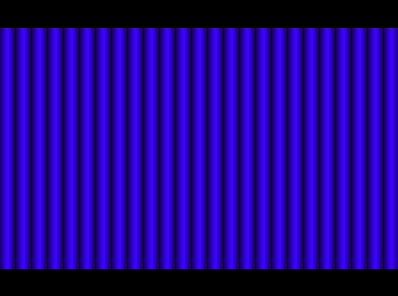
\includegraphics[width=\textwidth]{images/interface.png}
%\centering
%\caption{The Interface of Rational Piano after startup}
%\label{fig:interface}
%\end{figure}

%After the applet has been loaded, you see the interface like in Fig.\ref{fig:interface}.
After the applet has been loaded, you see just a black screen. The visualization will not appear until you provide some input to the system which then will look like in Fig.\ref{fig:interface_active}.

Now you can start playing around (but yet without sound or multitouch input): either click on the single lines or press your alphanumeric keyboard keys.

\textbf{Note:} The JAR has been complied for a \textbf{German Keyboard Layout}, if you want keyboard input for your differing keyboard layout, you need to recompile the application. But you are probably after Multitouch Input, so the keyboard layout does not matter anyway, it is just there for debugging purposes.

You should see a screen similar to Fig.\ref{fig:interface_active} when you press some keys. As long as a key is pressed, it is highlighted in a different color\footnote{green by default}.

\section{Setting Up MIDI Input}
\label{sec:midiinput}

Setting up MIDI input is easy in the newest version, as that can be done at runtime. After you have started \emph{Rational Piano}, you will see a dropdown control in the upper left corner of the screen. With a mouse click, you can change the MIDI input device which immediately can be used. The setting will be saved to the configuration file, so the next time you start \emph{Rational Piano}, that device will be used again.

\section{Setting Up Sound Output}
\label{sec:output}

To get Note Messages out of the Applet, one can either use MIDI or OSC (with namespace SynOSCopy). In either case a synthesizer application\footnote{or a host hosting VSTi plugins or whatever else understands one of the two communication protocols} is needed on the other side of that channel.

MIDI is the preferred way because nearly all software synthesizers understand it. OSC (and especially the SynOSCopy namespace) is not widely adopted for note messages to synthesizers.

\subsection{Using MIDI}

Java provides its own MIDI device ``Java Sound Synthesizer Sun Microsystems'' which supplies very ``cheap'' sounds without the need for program-external synthesizers. To activate that, edit the configuration file (on details see Sec.\ref{chap:settings}) and set ``outputMode = MIDI\_ONLY'' or ``outputMode = MIDI\_AND\_OSC'' and ``midiOutputDevice = Java Sound Synthesizer Sun Microsystems''\footnote{or just ``midiOutputDevice = java'' as partial strings are enough}.

When using this applet via MIDI with a \emph{software synthesizer}, one needs a \emph{Virtual MIDI Cable} to connect the Applet with the Synthesizer.

\emph{Maple Virtual Midi Cable} is a free one for Windows~\cite{bib:maple}. This specific virtual MIDI cable works simply: it has four ports that are registered as MIDI outputs and four ports that are registered as MIDI inputs. All data fed into one of those MIDI output ports gets forwarded to the corresponding MIDI input port.

In the configuration, you have to choose the correct MIDI output port according to your virtual MIDI cable. With \emph{Maple Virtual Midi Cable} this would be for example \emph{``Maple Midi Out: Port 4''}. You can adjust that to your needs in the configuration file, for more details see Chapter~\ref{chap:settings}.

That means, in your synthesizer application you need to setup the MIDI input to \emph{``Maple Midi In: Port 4''} or similar.

\textbf{Note:} If you have an \textbf{external} MIDI synthesizer connected to your soundcard via a physical MIDI cable, you \emph{do not} need the virtual MIDI cable. You just need to setup the hardware MIDI output port in the configuration file, for more details see chapter~\ref{chap:settings}.

\subsubsection{Help With the Synthesizer Application}

If you are desperate and do not know how to find a synthesizer application understanding MIDI, here is a little help. You also might head over to KVR~\cite{bib:kvr} and browse some free (or non-free) synthesizers. Note that for most of those, you will need a \emph{host application}.

A free VSTi\footnote{synthesizer plugin} for Windows and OSX is 4front Piano~\cite{bib:4front}.

But then you will still need a VST host application. A minimalistic free VST host is SAVIHost~\cite{bib:savi}, but it is only available for Windows. See its website for information on how to load a VST plugin (like 4front Piano) in SAVIHost.

To set the correct MIDI port in SAVIHost, in the Menu choose \emph{Devices $\rightarrow$ MIDI} and as \emph{Input Port} the entry \emph{``Maple Midi In: Port 4''} (or whatever your configured port is).

\textbf{Now you should be able to hear your playing from Rational Piano.} Do not forget to restart the application after installing the virtual MIDI cable.

\textbf{Info:} Furtherwise, under Windows, it is adviseable (but not necessary) to use an ASIO driver for the soundcard to achieve lower latency of the audio generating part. If you have a consumer audio card that does not ship with ASIO drivers, you can use ASIO4ALL~\cite{bib:asio4all}. Unfortunately SAVIHost does not support ASIO, but with other hosts you can minimize your audio latency that way.

\textbf{Alternative} to 4front Piano running in SAVIHost: You could also use PureData~\cite{bib:puredata}, but do not be too sad about poor sounding synths\footnote{You can make it sound good, but most simple synths just sound retro}. Start up PureData, activate the \emph{compute audio} checkbox, choose menu \emph{Help $\rightarrow$ Browser ...} then \emph{7.stuff/ $\rightarrow$ synth $\rightarrow$ 1.poly.synth.pd} which you need to double-click. Then choose menu \emph{Media $\rightarrow$ MIDI settings...} and as \emph{input device 1} choose \emph{Maple Midi In: Port 4}, press \emph{OK}. Now check that \emph{Edit} mode is \emph{deactivated} in menu \emph{Edit $\rightarrow$ Edit mode} (there should be no check mark next to the menu entry). Load a preset by clicking the circle next to \emph{recall} in one of the \emph{preset} boxes. Last thing to do is find the box next to \emph{MUTE} at the bottom of the patch and drag the number up to \emph{100}. That should be enough to let PureData receive MIDI messages from Rational Piano. If not, try activating the box on the top left of the patch under the text \emph{random note tester} which play some random notes. If not, check your audio settings in menu \emph{Media $\rightarrow$ Audio settings...}.


\subsection{Using OSC}

When using OSC, one has to use a host or synthesizer that understands OSC and the SynOSCopy namespace. You can use PureData~\cite{bib:puredata} with a custom patch for that task.

By default, OSC Voice messages get sent to UDP port \emph{12000} of \emph{localhost}.

\textbf{Note:} Rational Piano's Voice Management for SynOSCopy is not implemented yet due to a conceptual problem with SynOSCopy\footnote{If a voice gets turned off, the sender has no idea whether the synthesized voice has already faded out when it turns on the voice with the same number again. This could cut a fading-out voice. An idea for improvement for SynOSCopy would be to specify a parameter with the voice-on message which allows to choose whether the voice should be cut or not. The receiver then must have its own voice management.}. Right now, every note gets sent to the voice with the same number as the MIDI note number.

There is no polyphonic SynOSCopy patch for PureData yet. But you can try a monophonic one. Load up the \emph{Keyboard Example} from \emph{SynOscP5}~\cite{bib:synoscopy_keyboard_example}. In Edit mode\footnote{in menu \emph{Edit $\rightarrow$ Edit mode} there should be a check mark next to the menu entry}, change the box containing \emph{``routeOSC /V1''} to \emph{``routeOSC /*''}. Activate audio if you have not already by clicking menu \emph{Media $\rightarrow$ audio ON}. You can also turn up the volume with the green slider (with Edit mode deactivated).

\textbf{Now you should be able to hear your playing from Rational Piano.}


\section{Enabling Multitouch Input}
\label{sec:input}

Now, right after following the instructions of the last section, you should already be able to hear sounds when you press the typing keyboard keys.

Now we want to setup Multitouch Input from your multitouch table. You will need (or maybe already have) the program CCV (Community Core Vision)~\cite{bib:ccv}. Rational Piano was tested with CCV 1.3.

In CCV, adjust the camera recognition settings to your needs, and \textbf{activate TUIO UDP output} in the right panel in the section \emph{Communication}. This will by default map to TUIO port 3333 which is preconfigured in Rational Piano's settings.

This should be enough to make the Rational Piano application receive the multitouch messages generated by fingers pressing onto the surface. If it does not work as expected, examine the recognized blobs in CCV and try to adjust its settings.


\chapter{Tweaking the Settings}
\label{chap:settings}

When Rational Piano is run the first time, it generates a configuration file with filename \emph{``RationalPianoSettings.cfg''}. It is text-based and contains an explanation for each parameter which should be self-explanatory. You do not need to worry to mess anything up, the configuration file gets read everytime the application is started and immediately is written back in the original format again. All non-readable or garbage lines get sorted out. Parameters out of range get corrected, the minimum and maximum values are mentioned in the comments in the configuration file.

\textbf{Info:} For Double or Float values without a fractional, the dot is optional.

\section{Window Settings}

Settings to adjust window properties:

\noindent
\textbf{fullscreen} \\
\emph{Description:} Whether the application should get run full screen or in a window. \\
\emph{Note:} In full screen mode, the window width and height settings are ignored and the screen resolution is used instead. \\
\emph{Type:} Boolean. \\
\emph{Default value:} true.

\noindent
\textbf{vertical\_scaling} \\
\emph{Description:} Use the full width, but only the given fraction of the height of the full screen area, aligned to the bottom. \\
\emph{Note:} Only taken account for in fullscreen mode. This setting was set to 0.2 to produce the output seen in Fig.\ref{fig:interface_foto}. \\
\emph{Type:} Double. \\
\emph{Default value:} 1.0.

\noindent
\textbf{width} \\
\emph{Description:} Width of the application window's content. \\
\emph{Note:} Only in windowed mode. \\
\emph{Type:} Integer \\
\emph{Bounds:} Minimum = 100, Maximum = 10000. \\
\emph{Default value:} 1000.

\noindent
\textbf{height} \\
\emph{Description:} Height of the application window's content. \\
\emph{Note:} Only in windowed mode. \\
\emph{Type:} Integer \\
\emph{Bounds:} Minimum = 100, Maximum = 10000. \\
\emph{Default value:} 500.

\noindent
\textbf{framerate} \\
\emph{Description:} How often the image should get redrawn per second. The consonance calculation also takes place on every frame. \\
\emph{Type:} Float \\
\emph{Bounds:} Minimum = 1.0, Maximum = 200.0. \\
\emph{Default value:} 60.0.


\section{Line Settings}

\noindent
\textbf{notecount} \\
\emph{Description:} Counts of notes to display as lines. \\
\emph{Note:} The maximum MIDI note number is 127, so notestart + notecount - 1 should be smaller than 128. A full piano keyboard has 88 keys. \\
\emph{Type:} Integer \\
\emph{Bounds:} Minimum = 1, Maximum = 128. \\
\emph{Default value:} 88.

\noindent
\textbf{notestart} \\
\emph{Description:} MIDI note number of the first note. \\
\emph{Note:} The maximum MIDI note number is 127, so notestart + notecount - 1 should be smaller than 128. \\
\emph{Type:} Integer \\
\emph{Bounds:} Minimum = 0, Maximum = 127. \\
\emph{Default value:} 21 (A0).

\begin{figure}[!ht]
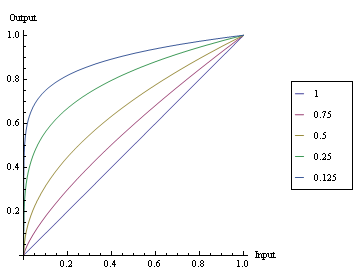
\includegraphics[width=0.7\textwidth]{images/linebend.png}
\centering
\caption{Nonlinear distortion of the line width translation}
\label{fig:linebend}
\end{figure}

\noindent
\textbf{lineBend} \\
\emph{Description:} Nonlinear distortion of the line width translation, 1 means no distortion, smaller values mean stronger distortion where the lines have a tendency to be more wide. \\
\emph{Note:} For a visual explanation how input values get translated to output values in dependence of this parameter, see Fig.\ref{fig:linebend}. \\
\emph{Type:} Double \\
\emph{Bounds:} Minimum = 0, Maximum = 1. \\
\emph{Default value:} 0.25.


\section{Note Output Settings}

\noindent
\textbf{outputMode} \\
\emph{Description:} Choose wheter Note messages should get sent via MIDI, OSC (with the SynOSCopy namespace), both or none. \\
\emph{Type:} Enum RationalPiano.NoteOut.outputModes  \\
\emph{Values:} MIDI\_ONLY, OSC\_ONLY, MIDI\_AND\_OSC, NO\_OUTPUT. \\
\emph{Default value:} NO\_OUTPUT.

\noindent
\textbf{oscport} \\
\emph{Description:} UDP port to send OSC voice messages (with the SynOSCopy namespace) to. \\
\emph{Type:} Integer \\
\emph{Bounds:} Minimum = 0, Maximum = 65535. \\
\emph{Default value:} 12000.

\noindent
\textbf{midiOutputDevice} \\
\emph{Description:} Part of the string of the MIDI port to send note messages to. \\
\emph{Note:} If you do not know the exact name of the port, just run the application and watch the debug output where all ports get listed. \\
\emph{Type:} String \\
\emph{Default value:} java.

\noindent
\textbf{midiInputDevice} \\
\emph{Description:} Part of the string of the MIDI port to receive note and sustain pedal messages from. \\
\emph{Note:} If you do not know the exact name of the port, just run the application and watch the debug output where all ports get listed. \\
\emph{Type:} String \\
\emph{Default value:} \emph{nothing}.

\noindent
\textbf{midiChannel} \\
\emph{Description:} MIDI channel to use for note messages that get sent to the chosen MIDI port. \\
\emph{Type:} Integer \\
\emph{Bounds:} Minimum = 0, Maximum = 15. \\
\emph{Default value:} 0.


\section{Consonance Calculation Settings}
\label{sec:ADSR}

\begin{figure}[!ht]
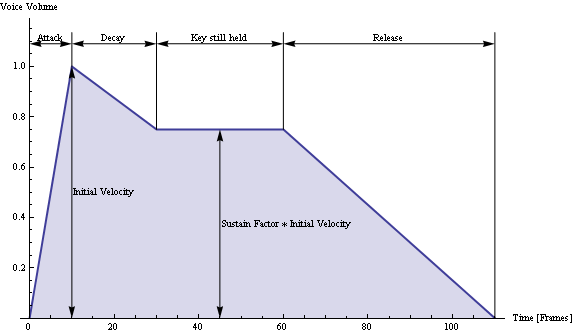
\includegraphics[width=\textwidth]{images/adsr_hold.png}
\centering
\caption{An ADSR (Attack Decay Sustain Release) curve in holdSustain mode where the key gets hold after the decay phase}
\label{fig:adsr_hold}
\end{figure}

\begin{figure}[!ht]
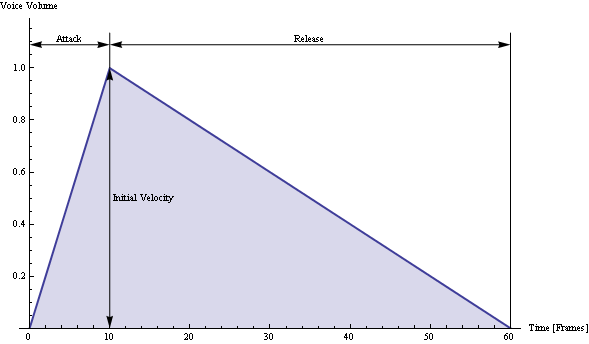
\includegraphics[width=\textwidth]{images/adsr_nohold.png}
\centering
\caption{An ADSR (Attack Decay Sustain Release) curve with deactivated holdSustain mode (pluck mode) where after the attack phase, the release phase follows immediately, no matter whether the key is still held}
\label{fig:adsr_nohold}
\end{figure}

For all pressed notes, internal volumes are tracked within the application for visualization purposes. To allow smooth visual transistions between note activations and deactivations, the volume of each activated note gets approximated by an ADSR (Attack Decay Sustain Release) curve. For two example ADSR curves, see Fig.\ref{fig:adsr_hold} and Fig.\ref{fig:adsr_nohold}. The volume curve is \textbf{not} meant to approximate the played sound of the synthesizer. It should approximate the fade-in and fade-out of the \textbf{felt presence} of a base frequency. So even when a note's sound has already been faded out physically, the human auditory system still tries to find consonant tones to that sound.

This is just for consonance calculation and does \textbf{not} impact note output.

\noindent
\textbf{attack} \\
\emph{Description:} Attack time of new voices in seconds. \\
\emph{Type:} Double \\
\emph{Bounds:} Minimum = 0, Maximum = 60. \\
\emph{Default value:} 0.15.

\noindent
\textbf{decay} \\
\emph{Description:} Decay time of held voices in seconds. \\
\emph{Note:} Only applicable if holdSustain is true. \\
\emph{Type:} Double \\
\emph{Bounds:} Minimum = 0, Maximum = 60. \\
\emph{Default value:} 4.0.

\noindent
\textbf{sustain} \\
\emph{Description:} Sustain level of held voices as a fraction of the initial velocity. \\
\emph{Note:} Only applicable if holdSustain is true, in that case the volume stays at the sustain level after the attack + decay phase. \\
\emph{Type:} Double \\
\emph{Bounds:} Minimum = 0, Maximum = 1. \\
\emph{Default value:} 0.0,  as the value of 0.0 results in a fadeout like with a piano sound when the value of decay is greater than that of release.

\noindent
\textbf{release} \\
\emph{Description:} Release time of held voices in seconds. \\
\emph{Type:} Double \\
\emph{Bounds:} Minimum = 0, Maximum = 60. \\
\emph{Default value:} 1.0.

\noindent
\textbf{holdSustain} \\
\emph{Description:} If true, hold the voices' volumes after attack + decay phase at the sustain level. If false, volumes are not held and release starts right after the attack phase (pluck mode). \\
\emph{Type:} Boolean \\
\emph{Bounds:} Minimum = 100, Maximum = 10000. \\
\emph{Default value:} true.

\noindent
\textbf{maxfrac} \\
\emph{Description:} Maximum dissonance to calculate a fraction for. \\
\emph{Note:} For details, see Chapter~\ref{chap:consonance}. \\
\emph{Type:} Integer \\
\emph{Bounds:} Minimum = 1, Maximum = 2147483647. \\
\emph{Default value:} 256 to include the \emph{just intonation} ratio of $\frac{16}{15}$.

\begin{figure}[!ht]
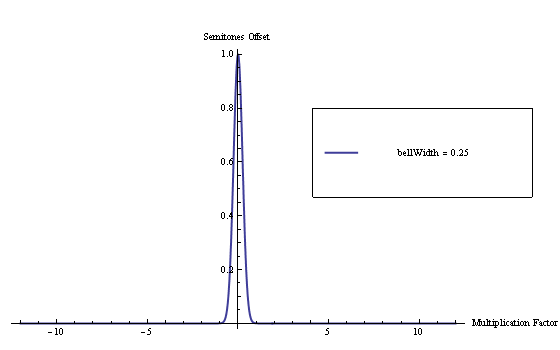
\includegraphics[width=\textwidth]{images/bellcurve.png}
\centering
\caption{Bell Curve with width = 0.25}
\label{fig:bellcurve}
\end{figure}

\noindent
\textbf{bellWidth} \\
\emph{Description:} Width of the bell curve which gets drawn around each fraction when calculating dissonance. \\
\emph{Note:} The bell curve has the function $e^{- \frac{(- 12 \cdot Log_2(fraction) + semitoneDifference)^2}{2 \cdot bellWidth^2}}$ like shown in Fig.\ref{fig:bellcurve}. \\
\emph{Type:} Double \\
\emph{Bounds:} Minimum = 0.01, Maximum = 1. \\
\emph{Default value:} 0.25.


\section{Multitouch Input Settings}

\noindent
\textbf{tuioPort} \\
\emph{Description:} UDP port to listen at for TUIO cursor messages. \\
\emph{Type:} Integer \\
\emph{Bounds:} Minimum = 0, Maximum = 65535. \\
\emph{Default value:} 3333.


\section{Color Settings}

The colors are setup in HSB format, so one color is expressed by the three 8-bit properties Hue, Saturation and Brightness.

\noindent
\textbf{backgroundColorHue} \\
\emph{Description:} Hue of the Background Color. \\
\emph{Type:} Integer \\
\emph{Bounds:} Minimum = 0, Maximum = 255. \\
\emph{Default value:} 0.

\noindent
\textbf{backgroundColorSaturation} \\
\emph{Description:} Saturation of the Background Color. \\
\emph{Type:} Integer \\
\emph{Bounds:} Minimum = 0, Maximum = 255. \\
\emph{Default value:} 0.

\noindent
\textbf{backgroundColorBrightness} \\
\emph{Description:} Brightness of the Background Color. \\
\emph{Type:} Integer \\
\emph{Bounds:} Minimum = 0, Maximum = 255. \\
\emph{Default value:} 0.

\noindent
\textbf{lineColorHueInactive} \\
\emph{Description:} Hue of an inactive line. \\
\emph{Type:} Integer \\
\emph{Bounds:} Minimum = 0, Maximum = 255. \\
\emph{Default value:} 180.

\noindent
\textbf{lineColorHueActive} \\
\emph{Description:} Hue of an active line. \\
\emph{Type:} Integer \\
\emph{Bounds:} Minimum = 0, Maximum = 255. \\
\emph{Default value:} 80.

\noindent
\textbf{lineColorSaturation} \\
\emph{Description:} Saturation of the color of a line. \\
\emph{Type:} Integer \\
\emph{Bounds:} Minimum = 0, Maximum = 255. \\
\emph{Default value:} 255.

\noindent
\textbf{lineColorBrightness} \\
\emph{Description:} Brightness of the color of a line. \\
\emph{Type:} Integer \\
\emph{Bounds:} Minimum = 0, Maximum = 255. \\
\emph{Default value:} 255.


\chapter{Understanding and Building the Sourcecode}
\label{chap:source}

\emph{Rational Piano} is open source, and can be found at \url{https://github.com/fabb/Rational-Piano}. All source files are well documented\footnote{in all conscience} with Javadoc. To read the generated Javadoc, open \emph{doc/javadoc/index.html}.

\section{Classes and How They Work Together}

To get a grasp of how the classes work together, they are visualized in an UML class diagram in Fig.\ref{fig:interaction}. Most classes are just instantiated once (in Fig.\ref{fig:interaction} all classes that have \emph{no} association with an ``0..*'' pointing at it).

\begin{figure}[htbp]
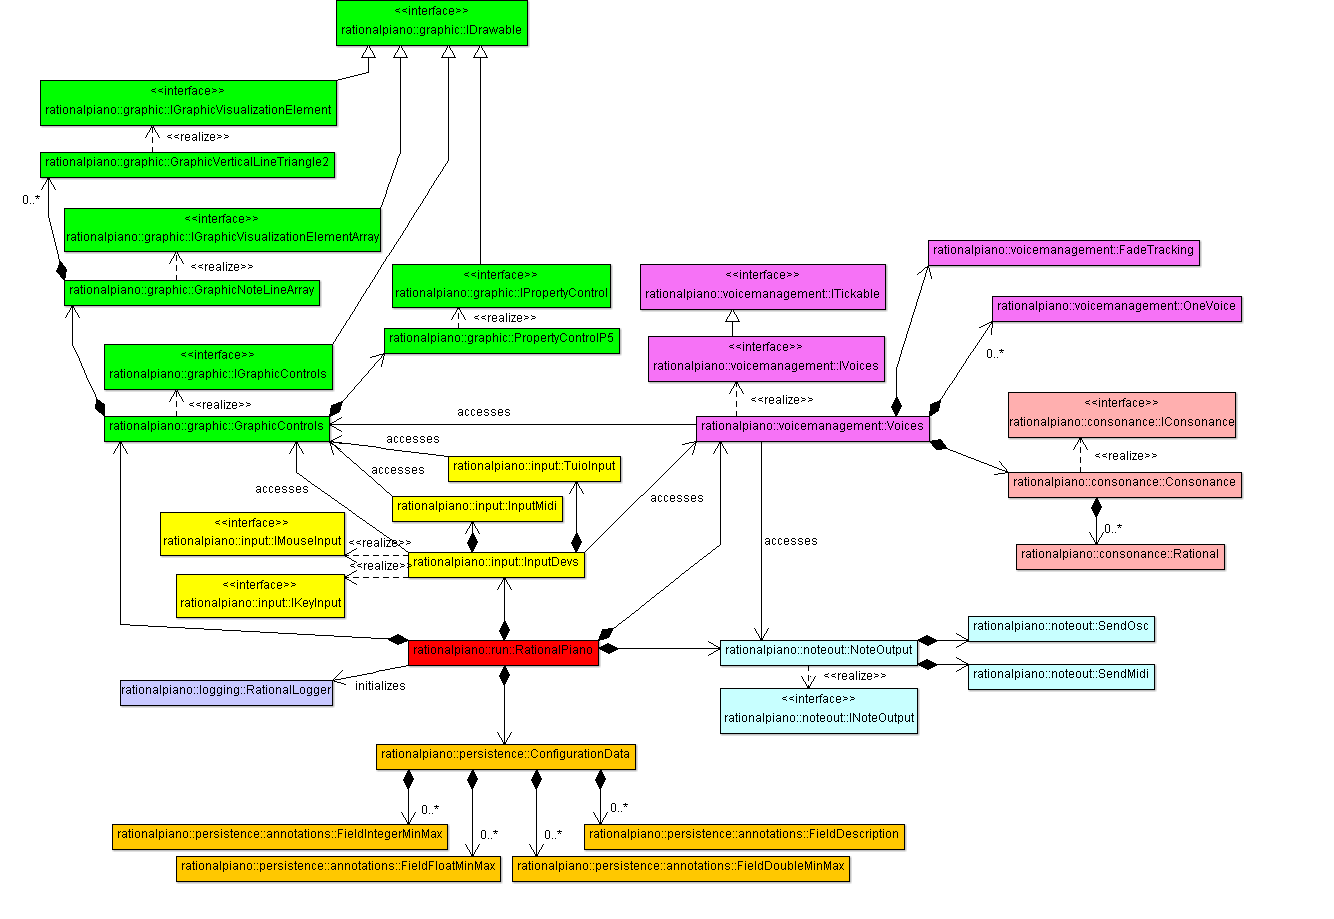
\includegraphics[width=\textwidth]{images/uml_class_diagram/rational_piano_class_diagram.png}
\centering
\caption{UML class diagram with associations between classes}
\label{fig:interaction}
\end{figure}


\subsection{rationalpiano.run}
\label{sec:Run}

\begin{itemize}
	\item \textbf{rationalpiano.run.RationalPiano} is the main class whose \emph{main()} method gets called to start the application. It is a Processing applet that gets called from itself with the method PApplet.main(). The advantage is that it can run both in \emph{present} mode\footnote{Processing's fullscreen mode} and as a native Java application.

	The class initializes the logger, loads the configuration, starts up the Processing applet and creates interconnected objects of GraphicControls, NoteOutput, Voices and InputDevs. Furthermore, it forwards Processing calls to draw() to the objects of GraphicControls (for drawing) and Voices (for consonance calculation). It also forwards keyboard and mouse events to the instance of InputDevs.
\end{itemize}


\subsection{rationalpiano.logging}

\begin{itemize}
	\item \textbf{rationalpiano.logging.RationalLogger} provides a method to initialize the top logger which gets (indirectly\footnote{The loggers of all other classes get routed through the top logger}) used for all debug output of the application. It is also possible to write all output to a logfile by initializing the logger with a different parameter.
\end{itemize}


\subsection{rationalpiano.persistence}

\begin{itemize}
	\item \textbf{rationalpiano.persistence.ConfigurationData} holds several public fields that are the initialization parameters for the generated objects mentioned in Section~\ref{sec:Run}. For an explanation of all fields, refer to the full documentation of \emph{Rational Piano}~\cite{bib:RationalPianoDoc}. The class is able to read in the configuration from a file in combination with sanitizing the read data and also writing the configuration to a file again.
\end{itemize}


\subsection{rationalpiano.persistence.annotations}

\begin{itemize}
	\item This package contains the annotations \textbf{FieldDescription}, \textbf{FieldDoubleMinMax}, \textbf{FieldFloatMinMax} and \textbf{FieldIntegerMinMax} which are used to comment the fields of rationalpiano.persistence.ConfigurationData in a way that it is possible to write the comments to the configuration file.
\end{itemize}


\subsection{rationalpiano.voicemanagement}

\begin{itemize}
	\item \textbf{rationalpiano.voicemanagement.Voices} manages active voices. It provides methods to add and remove voices which get called by an object of InputDevs. Voices also keeps an instance of Consonance with which it calculates the consonance for all active voices every frame. The resulting consonances get sent to the according GraphicVerticalLineTriangle2 objects fetched from the object of GraphicControls to set the line widths. The class implements the interface \textbf{rationalpiano.voicemanagement.IVoices} which itself extends the interface \textbf{rationalpiano.voicemanagement.ITickable}. IVoices provides access from InputDevs and ITickable allows to advance the single voices' time by the class RationalPiano.

	\item Every active voice is an object of type \textbf{rationalpiano.voicemanagement.OneVoice} that allows to store various parameters like initial velocity or hold time individually for each active voice. 

	\item \textbf{rationalpiano.voicemanagement.FadeTracking} makes it possible to use an ADSR\footnote{Attack Decay Sustain Release - More information on this can be found in~\cite{bib:RationalPianoDoc}} envelope for each voice. The Voices object uses an object of this class to calculate a current velocity for each active voice by passing the according OneVoice object.
%%TODO \footnote{see Section~\ref{sec:ADSR}}
\end{itemize}

\subsection{rationalpiano.consonance}

\begin{itemize}
	\item \textbf{rationalpiano.consonance.Consonance} provides a method to calculate the consonance for all keys in range for a set of voice velocities. The Consonance class implements the interface \textbf{rationalpiano.consonance.IConsonance} which is used for access by the Voices object which initializes and keeps an instance of Consonance. For an explanation of the computation, see Section~\ref{sec:computation}.

	\item \textbf{rationalpiano.consonance.Rational} represents a rational number and is used for the initialization of Consonance.
\end{itemize}


\subsection{rationalpiano.graphic}

\begin{itemize}
	\item \textbf{rationalpiano.graphic.GraphicControls} manages the screen elements\footnote{background, line visualization and parameter control} and allows to draw them with a provided method. It holds an instance of GraphicNoteLineArray and PropertyControlP5. The class implements \textbf{rationalpiano.graphic.IGraphicControls} which itself extends the interface \textbf{rationalpiano.graphic.IDrawable}. IGraphicControls provides access to the contained GraphicNoteLineArray for an object of Voices, InputDevs, TuioInput and InputMidi.

	\item \textbf{rationalpiano.graphic.GraphicNoteLineArray} holds all GraphicVerticalLine objects drawn on the screen. It distributes them across the screen and manages their corresponding MIDI keys. The class implements \textbf{rationalpiano.graphic.IGraphicVisualizationElementArray} which itself extends the interface \textbf{rationalpiano.graphic.IDrawable}. IGraphicVisualizationElementArray provides methods for querying contained line objects by objects of Voices, InputDevs and TuioInput.

	\item \textbf{rationalpiano.graphic.GraphicVerticalLineTriangle2} represents a vertical line that has a changeable volume\footnote{volume means visual ``intensity'' and results in a changed height, width and color} and activation state. It provides a method to get drawn on screen. The class implements \textbf{rationalpiano.graphic.IGraphicVisualizationElement} which itself extends the interface \textbf{rationalpiano.graphic.IDrawable}. IGraphicVisualizationElement provides methods to change the line's volume and activation state to be accessed by an object of the class Voices.
	
	\item \textbf{rationalpiano.graphic.PropertyControlP5} provides on-screen control elements which can be tweaked with the mouse and change configuration parameters at runtime\footnote{in the current version, there only is one dropdown menu implemented to change the MIDI input device}. A changed parameter will be propagated to the object of ConfigurationData and the configuration will be saved to the settings file. The class implements \textbf{rationalpiano.graphic.IPropertyControl} which itself extends the interface \textbf{rationalpiano.graphic.IDrawable}. IPropertyControl provides methods to add controllable objects\footnote{in the current version an object of InputMidi} and to query whether the mouse hovers a control element to avoid clicks on parameter controls to affect the line visualization.
\end{itemize}


\subsection{rationalpiano.input}

\begin{itemize}
	\item \textbf{rationalpiano.input.InputDevs} manages input from mouse and keyboard. For multitouch it creates an object of TuioInput. For MIDI input it creates an object of InputMidi. For each new input it looks up the corresponding MIDI key in the GraphicControls object and then activates or deactivates the according voice with a call to the Voice object. It also sends the input to the NoteOut object. The class implements the interfaces \textbf{rationalpiano.input.IKeyInput} and \textbf{rationalpiano.input.IMouseInput} which take mouse and keyboard input from the RationalPiano class.

	\item \textbf{rationalpiano.input.TuioInput} manages TUIO input and processes it the same way as InputDevs.
	
	\item \textbf{rationalpiano.input.InputMidi} manages MIDI input and processes it the same way as InputDevs. Supported MIDI messages are \emph{note on}, \emph{note off} and \emph{damper pedal CC messages}.
\end{itemize}


\subsection{rationalpiano.noteout}

\begin{itemize}
	\item \textbf{rationalpiano.noteout.NoteOutput} sets up MIDI and SynOSCopy output according to the configuration. It provides functions to activate and deactivate a note/voice and send sustain (damper pedal) messages. It forwards those calls to SendMidi and/or SendOsc, depending on the configuration. The class implements the interfaces \textbf{rationalpiano.noteout.INoteOutput} which is used by InputDevs, TuioInput and InputMidi to control output note messages.

	\item \textbf{rationalpiano.noteout.SendMidi} opens the configured MIDI device and forwards note messages to it.

	\item \textbf{rationalpiano.noteout.SendOsc} forwards note messages to the configured UDP port as a SynOSCopy message.
\end{itemize}


\section{Library Dependencies}
\label{sec:libdep}

The application relies on Java, Processing and some additional libraries for control element, MIDI, SynOSCopy and TUIO support.

The necessary libraries\footnote{except to the JDK} are included in the subdirectory \emph{lib}. All of them are open source. For the exact licenses, see the following sections.


\subsection{Java Development Kit}

You will need a Java SE Development Kit~\cite{bib:jdk} with version 6 or later. Version 5 probably would work too, but it was not tested.


\subsection{Processing}

The library \emph{core.jar} included with Processing is needed~\cite{bib:processing}. This application was tested with versions 1.0, 1.1 and 1.2.1, no changes were necessary to run it with the diverse versions. 

\noindent
The used export library is licensed under the GNU LGPL~\cite{bib:lgpl}.


\subsection{controlP5}

For control elements on-screen, like the dropdown to select the MIDI input device, the controlP5 library \emph{controlP5.jar} with version 0.5.4 is used~\cite{bib:controlP5}.

\noindent
The library is licenced under the GNU LGPL~\cite{bib:lgpl}.


\subsection{TUIO}

For multitouch input, the TUIO library \emph{libTUIO.jar} with version 1.4 is used~\cite{bib:tuio}.

\noindent
The library is licenced under the GNU GPL version 2~\cite{bib:gpl2}.


\subsection{RWMidi}

For MIDI in- and output, the library \emph{rwmidi.jar} with version 0.1c is used~\cite{bib:rwmidi}.

\noindent
It is licensed under the GNU LGPL~\cite{bib:lgpl}.


\subsection{SynOscP5}

For SynOSCopy output, the libraries \emph{javaosc.jar} and \emph{synOscP5.jar} with versions from 12 September 2009 are used~\cite{bib:synoscopy}.

\noindent
The library \emph{synOscP5.jar} is licensed under the Artistic License~\cite{bib:artistic}.

\noindent
The exact copyright notice and license text for the library \emph{javaosc.jar} is stated in file \emph{lib/javaosc\_license.txt}.


\chapter{Prospects and Future Development Ideas}
\label{chap:future}

Some of the listed bugs or ideas might be outdated. The current state can be found in the issue tracker at \url{https://github.com/fabb/Rational-Piano/issues}. 


\section{Bugs}

There are some lines marked in the sourcecode with the keywords \textbf{TODO}, \textbf{FIXME} and maybe also \textbf{XXX}. Next to TODO or FIXME there should be a description for what is to do or to fix. XXX usually stands for a missing Javadoc comment.

\begin{itemize}
	\item \textbf{Problem:} The RWMidi Library does not throw exceptions. So when opening an unavailable MIDI device, a stack trace gets printed out, but the program continues normally, unaware of the failed attempt. Everytime a MIDI message gets sent to the unopened device, a new stack trace gets printed. \\
	\textbf{Solution:} Modify the open source library RWMidi and throw exceptions instead of catching them and printing stack traces.

	\item \textbf{Problem:} If two blobs get too close, they merge and generate a new blob with a new note-on message.
\end{itemize}


\section{Expansions}


\subsection{Display and Interface}

\begin{itemize}

	\item Provide a \textbf{Menu} to adjust parameters online. Done for MIDI input for now.
	
	\item Calculate \textbf{Overall Consonance} of the playing and display it e.g. by a varying background color.

	\item Provide an additional \textbf{Visual Output} of active voices' nearest rational numbers in a prime factor view or in divisor tree view.

\end{itemize}


\subsection{Input}

\begin{itemize}

	\item Make \textbf{Keyboard-Input localized} and not just for the German Layout.

	\item A \textbf{``Tutor'' Mode} where musical pieces or harmony series get played back that also do not get routed to the note output.

	\item \textbf{Polyphonic Pitch-Shift} where a moving finger changes the frequency of the corresponding note. The frequencies where the note snaps could either be keys of a fixed scale or follow different algorithms (see next idea). \\
	\textbf{Problems:} It is hard for the framework to do the tracking of crossing fingers, errors are possible. MIDI messages would need pitch bend which only works with a channel hack.

	\item \textbf{Snap Setting} for polyphonic pitch-shift - for example the voices could snap to at least equal-consonant frequencies as the first touch, or another example is a controller (like a foot pedal) to adjust the snap width.

	\item Introduce the possibility of an \textbf{Interconnection of several Multotouch Tables} which are all separate keyboard controllers by themselves, but whose consonance calculation takes account for active voices of the other tables.

\end{itemize}


\subsection{Consonance Calculation}

\begin{itemize}

	\item The consonance calculation formula could get tweaked a little so that the fade-out looks smoother at the end.

	\item ADSR values could be relative delta-values. \\
	\textbf{Benefit:} The attack-/decay-/release-\textbf{rate} and not the time is the same for all voices. \\
	\textbf{Problem:} The voices then are no more stateless as they must know in which phase they are, there is no possibility to determine the phase just from the frame-age of the voice anymore.

	\item Take account for the \textbf{Spectrum of the Sound Generator} for calculating the consonance\footnote{William Sethares developed such an approach with his ``Adaptive Tuning''}. This could either be achieved with static samples of the synthesizer or with dynamically recorded ones.

	\item An expansion of the previous idea would be to record the environment and provide the possibility to play \textbf{consonant to the ambient}.

\end{itemize}


\subsection{Scales}

\begin{itemize}

	\item Use different (fixed) \textbf{Scales} than 12TET. \\
	\textbf{Difficulty:} MIDI Tuning messages or MIDI Pitch Bend messages would be necessary.

	\item Provide a \textbf{Continuous Scale}\footnote{A bit like the Continuum Fingerboard~\cite{bib:continuum}} as input. Pressed x-values ``snap'' to a next consonant ratio. The minimum consonance could be set in real time by a parameter (controlled e.g. by a foot pedal). \\
	\textbf{Difficulty:} MIDI messages would need pitch bend which only works with a channel hack.

\end{itemize}


\subsection{Dreams}

\begin{itemize}

	\item An \textbf{Automatic Mode} where a very harmonic playing or accompaning takes place would be an ultimate goal. This is very hard as also the dimension of rhythm has to be considered.

\end{itemize}


% appendices
\appendix
%\input{app1}

\chapter{History of Changes}
\label{chap:history}

\indent
\textbf{2011-02-04}

Renewed the documentation to reflect additions of MIDI input and some other things.

\textbf{2010-07-30}

First public release.


\clearpage
\phantomsection
\addcontentsline{toc}{chapter}{References}

\bibliographystyle{plain}

\nocite{*}

%\bibliography{bla}

\begin{thebibliography}{99}

\bibitem{bib:consonance}
  \emph{Consonance} Wikipedia entry.
  \url{http://en.wikipedia.org/wiki/Consonance}.

\bibitem{bib:midi}
  \emph{MIDI} Wikipedia entry.
  \url{http://en.wikipedia.org/wiki/Midi}.

\bibitem{bib:osc}
  \emph{OSC}.
  \url{http://opensoundcontrol.org/}.
  
\bibitem{bib:sethWiki}
  William Sethares,
  \emph{Wikipedia entry}.
  \url{http://en.wikipedia.org/wiki/William_Sethares}.

\bibitem{bib:adaptun}
  William Sethares,
  \emph{Adaptive Tuning}.
  \url{http://eceserv0.ece.wisc.edu/~sethares/paperspdf/adaptun.pdf}.

\bibitem{bib:12tet}
  \emph{Equal Temperament} Wikipedia entry.
  \url{http://en.wikipedia.org/wiki/Equal_temperament}.

\bibitem{bib:just}
  \emph{Just Intonation} Wikipedia entry.
  \url{http://en.wikipedia.org/wiki/Just_intonation}.

\bibitem{bib:bell}
  \emph{Gaussian Bell Curve} Wikipedia entry.
  \url{http://en.wikipedia.org/wiki/Gaussian_function}.
  
\bibitem{bib:cent}
  \emph{Musical Cent} Wikipedia entry.
  \url{http://en.wikipedia.org/wiki/Cent_(music)}.

\bibitem{bib:factorization}
  \emph{Prime Factorization} Wikipedia entry.
  \url{http://en.wikipedia.org/wiki/Prime_factorization}.

\bibitem{bib:cons_diss}
  \emph{Consonance and Dissonance} Wikipedia entry.
  \url{http://en.wikipedia.org/wiki/Consonance_and_dissonance}.

\bibitem{bib:harmonic_entropy}
  \emph{Harmonic Entropy} Model.
  \url{http://launch.groups.yahoo.com/group/harmonic_entropy/}.

\bibitem{bib:mathematica}
  \emph{Wolfram Mathematica} Homepage.
  \url{http://www.wolfram.com/products/mathematica/index.html}.

\bibitem{bib:dia}
  \emph{Dia} Homepage.
  \url{http://live.gnome.org/Dia}.

\bibitem{bib:java}
  \emph{Java Runtime Environment (JRE) Download}.
  \url{http://www.java.com/en/download/manual.jsp}.

\bibitem{bib:jdk}
  \emph{Java SE Development Kit (JDK) 6 Download}.
  \url{http://java.sun.com/javase/downloads/widget/jdk6.jsp}.
  
\bibitem{bib:maple}
  \emph{Maple Virtual Midi Cable}.
  \url{http://www.maplemidi.com/Maple_driver.html}.
  
\bibitem{bib:4front}
  \emph{4front Piano VSTi}.
  \url{http://www.yohng.com/piano.html}.
  
\bibitem{bib:kvr}
  \emph{KVR}.
  \url{http://www.kvraudio.com/}.
  
\bibitem{bib:asio4all}
  \emph{ASIO4ALL}.
  \url{http://www.tippach.net/asio4all}.
  
\bibitem{bib:savi}
  \emph{SAVIHost} free VST Host.
  \url{http://www.hermannseib.com/english/savihost.htm}.
  
\bibitem{bib:puredata}
  \emph{PureData}.
  \url{http://puredata.info/downloads}.
  
\bibitem{bib:ccv}
  \emph{CCV (Community Core Vision)}.
  \url{http://ccv.nuigroup.com/}.

\bibitem{bib:processing}
  \emph{Processing Download}.
  \url{http://processing.org/download/}.

\bibitem{bib:controlP5}
  \emph{controlP5}.
  \url{http://www.sojamo.de/libraries/controlP5/}.

\bibitem{bib:rwmidi}
  \emph{RWMidi}.
  \url{http://ruinwesen.com/files}, \url{http://ruinwesen.com/support-files/rwmidi-0.1c.zip}.
  Documentation: \url{http://ruinwesen.com/support-files/rwmidi/documentation/RWMidi.html}.

\bibitem{bib:tuio}
  \emph{TUIO Download}.
  \url{http://www.tuio.org/?software}, Direct Download at \url{http://prdownloads.sourceforge.net/reactivision/TUIO_JAVA-1.4.zip?download}, Javadoc at \url{http://www.tuio.org/?java}.
  
\bibitem{bib:synoscopyNamespace}
  \emph{SynOSCopy Namespace Proposal}.
  \url{http://github.com/fabb/SynOSCopy/wiki}.

\bibitem{bib:synoscopy}
  \emph{SynOSCopy}.
  \url{http://code.google.com/p/synoscp5/} and \url{http://51858360.de.strato-hosting.eu/synoscp5/}.
  
\bibitem{bib:synoscopy_keyboard_example}
  \emph{SynOSCopy Keyboard Example}.
  \url{http://51858360.de.strato-hosting.eu/synoscp5/keyboard.html} and a direct link to the PureData patch: \url{http://51858360.de.strato-hosting.eu/synoscp5/examples/keyboard/keyboard.pd}.
  
\bibitem{bib:osl}
  \emph{Open Software License (``OSL'') v. 3.0}.
  \url{http://www.opensource.org/licenses/osl-3.0.php}.

\bibitem{bib:lgpl}
  \emph{GNU Lesser General Public License}.
  \url{http://www.opensource.org/licenses/lgpl-license.php}.

\bibitem{bib:gpl2}
  \emph{GNU General Public License version 2}.
  \url{http://www.opensource.org/licenses/gpl-2.0.php}.
  
\bibitem{bib:artistic}
  \emph{Artistic License}.
  \url{http://dev.perl.org/licenses/artistic.html}.

\bibitem{bib:continuum}
  \emph{Continuum Fingerboard}.
  \url{http://www.cerlsoundgroup.org/Continuum/}.

\end{thebibliography}

\end{document}
